% !TeX root = ../main.tex

\chapter{系统概要设计}
本章叙述了CI/CD流水线调度系统的设计。
首先介绍了系统的总体设计和架构分层,随后分别叙述系统内各个模块的设计与其之间的连接,
然后后对系统的数据库从概念设计和逻辑设计两方面进行了阐述,最后对本小节内容进行了总结。

\section{系统总体设计}

在对整个CI/CD流水线调度系统进行需求分析后,可以发现本系统的功能业务复杂且对部分服务的横向扩展有着较高需求。
可将本系统的核心模块拆分为三个微服务,分别为Backend服务、调度器服务和执行器服务,每个服务下又包含一些子模块。
进行这样服务划分的目的是降低系统间各模块的耦合性,并为不同的模块分配合适的资源,方便不同的模块分别以多节点的方式进行部署。
同时,拆分后的服务借助容器调度系统Kubernetes,可以实现弹性扩容和故障转移。
系统架构图如图~ \ref{fig:系统架构图}

\begin{figure}[h]
  \centering
  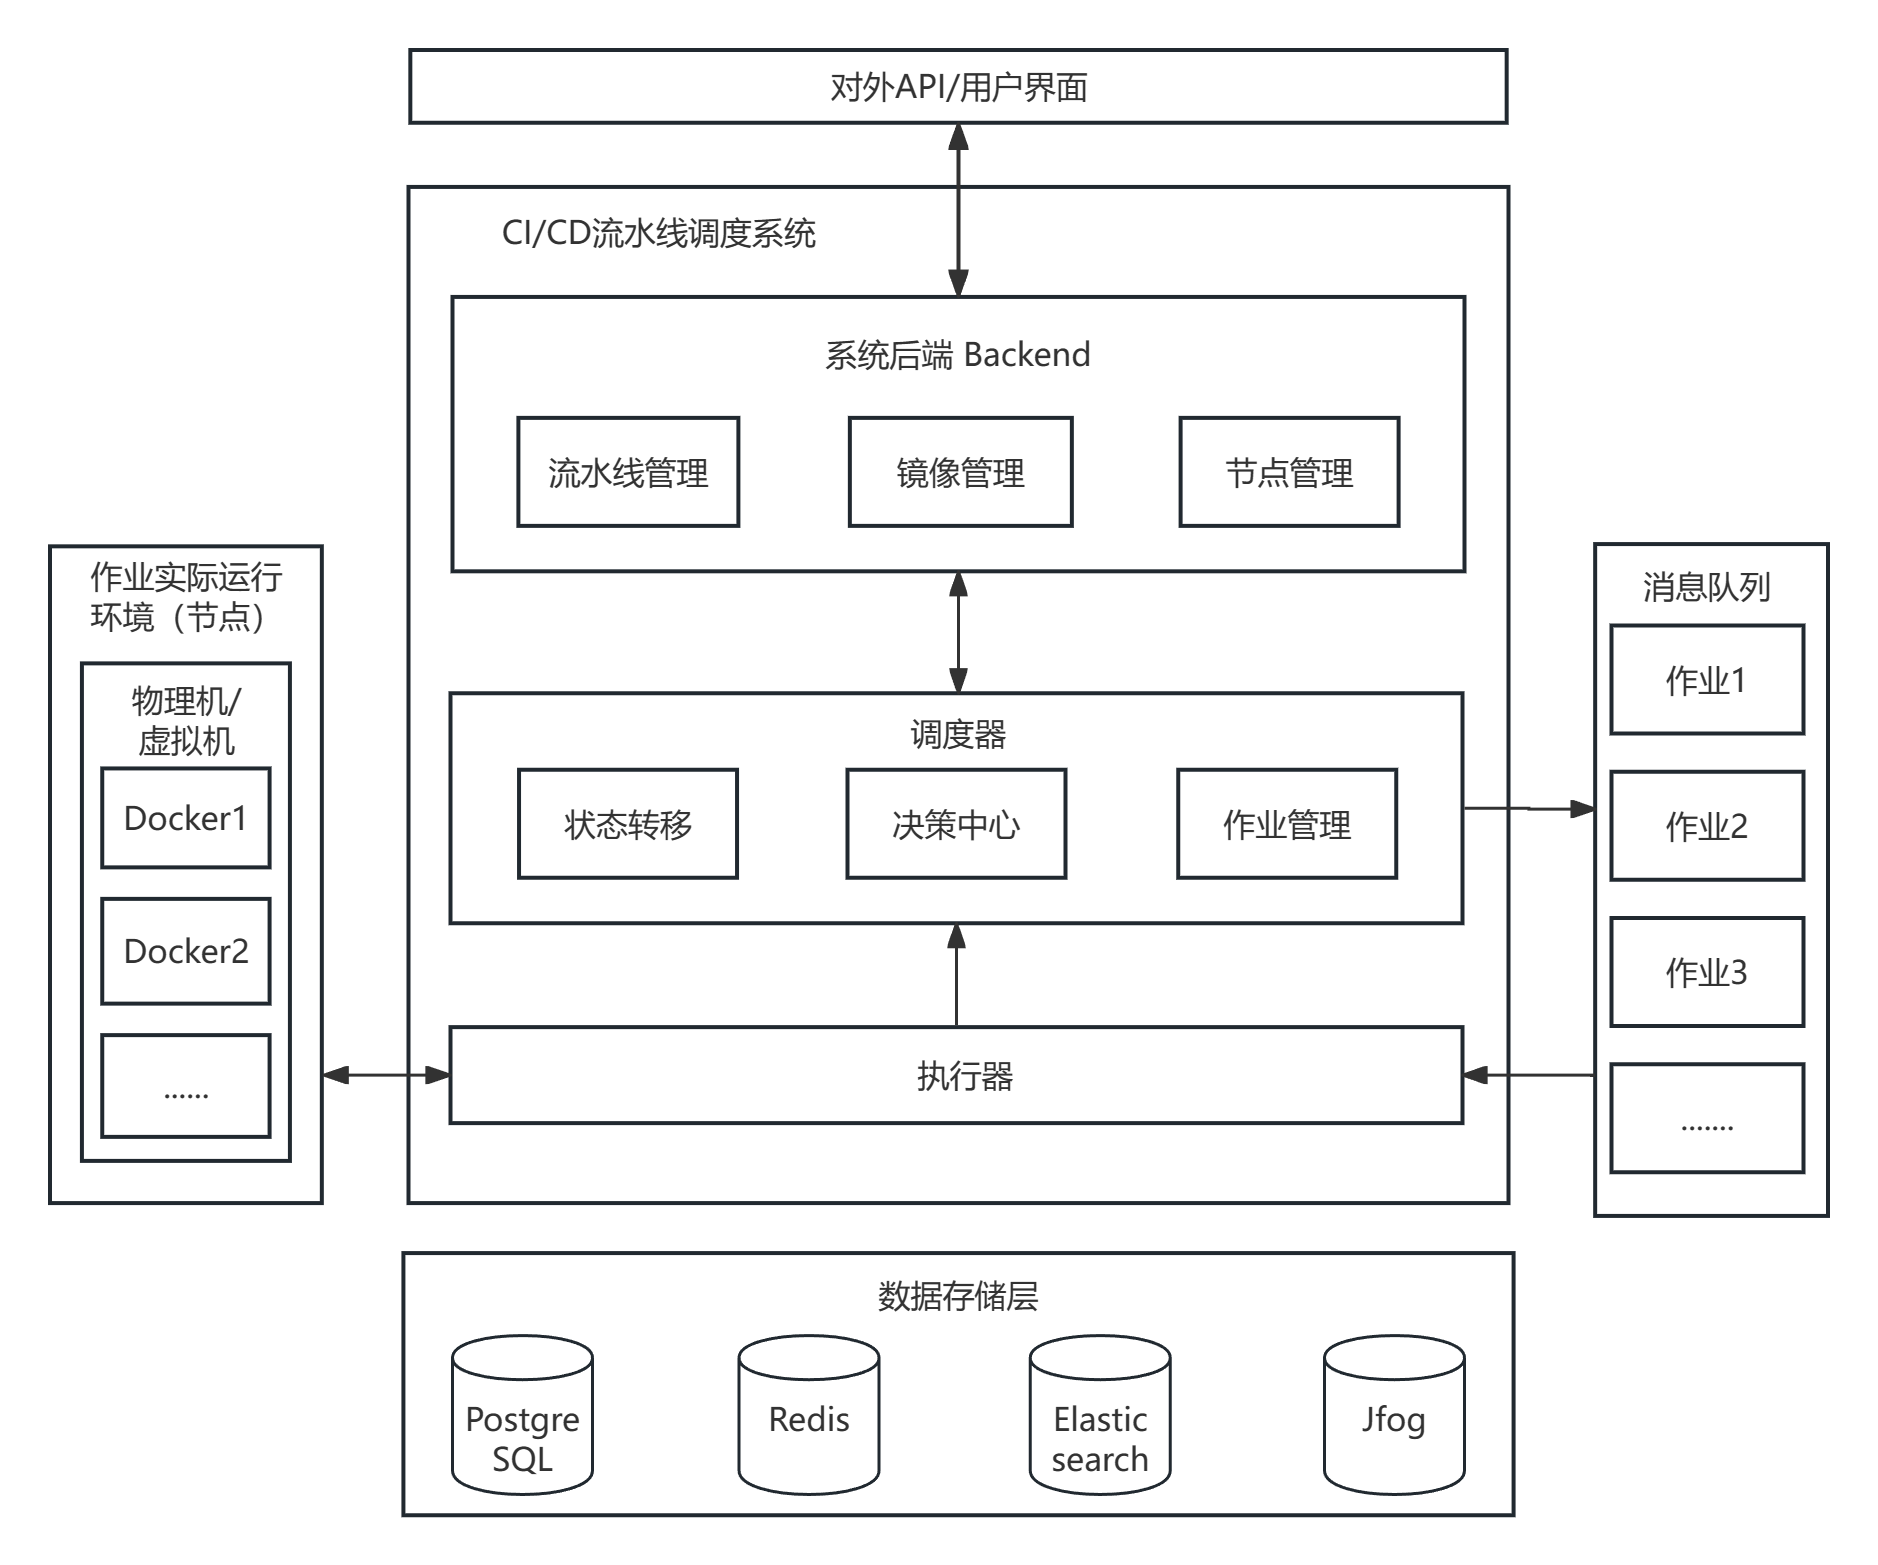
\includegraphics[width=1\textwidth]{流水线系统架构图.png}
  \caption{系统架构图}
  \label{fig:系统架构图}
\end{figure}

首先最上层是对外公开的api和前端UI,用户将通过该层与

系统内部同一时刻将有许多流水线作业同时执行,调度器负责流水线中各个子概念的状态切换,同时依据不同流水线的配置和状态来对当前流水线作业的调度进行决策,将需要被执行的作业交付给执行器模块。
执行器则最终负责各个流水线作业的真实执行,将作业转换为真正的可执行程序或者脚本后在真实的运行环境(Docker、物理机或虚拟机)中执行,并实时监控中运行环境中作业的运行状态,反馈给调度器。



\section{系统模块设计}
把每个模块讲一下:加入数据流图描述作业数据的流动。

\subsection{Backend}

首先是Backend模块,系统通过该模块向外部暴露API以供前端/外部接口调用。
用户在前端进行的操作、填写的配置信息等将通过API接口传递给Backend模块,Backend模块接收到数据后,会进行相应的业务逻辑处理,如对用户创建的流水线进行合法性校验、对作业数据进行合法性校验等,最后负责将数据落库。
同时,在流水线运行过程中,用户对流水线的手动干预操作,也是先调用接口传递给Backend模块,然后再由Backend模块进行一定处理后传递给调度器模块,用户界面与调度器模块完全解耦。

Backend有以下三种典型服务场景:

当用户通过API接口传入如“取消”、“跳过”、“人工审核通过”等人工干预命令时,Backend会根据权限模型对用户进行鉴权,如只有流水线的拥有者才有权干预流水线、只有预设的审核人才有权进行人工审核等。
通过鉴权后,Backend将对人工干预命令进行进一步封装,携带一些额外的信息后,将命令发送给调度器模块,由调度器对流水线的执行进行真正的干预。

当用户通过API接口创建或编辑流水线时,Backend会对流水线的内容进行解析,并通过序列化器对内容进行合法性校验,然后将流水线以阶段、作业和任务的维度进行分拆,
并将拆解后的流水线数据持久化进数据库。

当用户通过API接口触发流水线时,Backend将从数据库中获取流水线数据,进行一定封装后发送给调度器模块。
随后,调度器会不断地向Backend返回流水线的执行信息,以便Backend实时更新流水线的运行状态。
与此同时,Backend会接收到前端的轮询请求,用以实时展示给用户。


\subsection{调度器(CI-Master)}

调度器模块是整个系统的核心模块,其中包含状态转移、决策中心与作业管理三个子模块,分别介绍如下:

\subsubsection{状态转移}



\subsubsection{决策中心}

\subsubsection{作业管理}



\subsection{执行器(CI-Runner)}

执行器的设计目的是为了能够稳定高效地执行不同类型的作业,以待执行的作业信息为输入,以作业执行结果为输出,并且支持快速横向扩展,提高作业执行能力。
作业执行器首先需要能够根据自身能够执行的作业类型获取与之相对应的作业。
获取作业之后,能够保证顺利且高效的完成作业执行。
在执行完毕后,将作业状态上报给调度器。
执行器本系统将使用开源的Gitlab Runner,GitLab Runner在Gitlab的CI/CD模块中也扮演执行器的功能,并且与Gitlab主模块使用Http Apis进行通信,本系统中将对这些Http Apis进行抓包,获得这些Api的Url以及出入参后,便可如法炮制地将本系统的调度器接入GitLab Runner。
为了保证系统的稳定性,流水线执行器将部署在Kubernetes中,流水线执行器可以根据当前CI/CD的资源需求自动创建或删除副本(在Kubernetes称作Pod),以适应负载的变化:当系统进入使用高峰期时,系统可以自动创建更多的执行器副本来处理请求,而当负载减少时,多余的副本会被自动删除,从而实现资源的高效利用;
同时,当某个执行器发生故障时,Kubernetes会自动检测到故障,并将受影响的CI/CD负载迁移到其他健康的执行器副本上,避免应用程序中断或停止对外提供服务,提高系统稳定性。


\subsection{消息队列}

本系统调度器与执行器之间的消息交互是借助一个消息队列来完成的,本系统中使用阿里巴巴开发的RocketMq 5.0。
当调度器封装好一个流水线作业运行实例时,调度器将作为消息队列的生产者,将作业运行实例放入队列中;执行器作为消息队列的消费者,将持续消费队列中的消息。
调度器和执行器分别与消息队列进行交互,两者之间解耦,便于后续扩展。

系统引入消息队列的主要目的是实现需求分析中的\nameref{subsec:流水线作业合理调度需求}。
首先,消息队列先进先出的特性能够保证执行器有序地消费作业运行实例,避免了程序异步执行带来的作业执行顺序错乱问题,使得作业的执行严格按照调度器预设的顺序执行。
并且,当系统使用高峰期来临,作业量超过了执行器的负载能力时,消息队列承担了缓冲的作用,来不及被消费的作业将按照顺序被堆积在消息队列中,等到执行器处理完当前作业,具备处理能力后,再去消息队列的队头中拉取作业。

调度器、执行器与消息队列之间的时序图如图\ref{fig:消息队列时序图}

\begin{figure}[h]
  \centering
  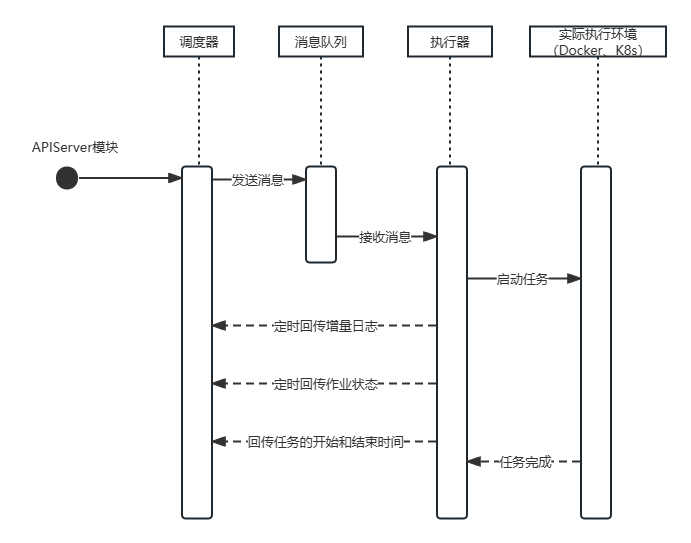
\includegraphics[width=0.8\textwidth]{消息队列时序图.png}
  \caption{调度器、执行器与消息队列间时序图}
  \label{fig:消息队列时序图}
\end{figure}

\subsection{数据存储层}
数据存储层是对本系统中各个数据和文件存储服务的抽象,负责整个系统所有数据的持久化服务。
包括流水线以及其子概念的配置信息、运行记录、Docker镜像、作业执行产物(如编译后压缩产生的tar包等)以及作业运行日志等。


本系统中,使用PostgreSQL存储流水线的配置和运行记录的相关数据,这部分数据属于结构化数据,数据字段和格式较为固定,故采用业界主流的关系型数据库进行存储和管理;
使用Redis存储缓存信息,加快接口的响应速度,提升用户体验;
JFrog Artifactory存储镜像管理模块涉及到的Docker镜像,以及流水线任务执行完成后的执行产物,比如单元测试报告等;
日志平台建立在 Elastic Search 之上,用于集中记录整个系统的所有运行日志,所有子系统的日志都会传送至该平台进行聚合。
其具体原理与功能与本系统主体功能无关,不再赘述。

上述不同类型的数据及其存储方式总结如表\ref{tab:系统数据存储方式}所示.

\begin{table}[h]
  \centering
  \caption{系统数据存储方式}
  \label{tab:系统数据存储方式}
  \begin{tabular}{clll}
    \toprule
    数据类型 & 主要内容      & 存储方式   & 选型 \\
    \midrule
    结构化数据     & 配置信息和运行记录      & 关系型数据库   & PostgreSQL       \\
    缓存数据       & 接口响应数据                   & 键值存储   & Redis       \\
    二进制数据     & Docker镜像、流水线任务执行产物  & 二进制数据管理系统   & JFrog Artifactory   \\
    日志数据       & 日志                & 分布式日志系统  & Elastic Search       \\
    \bottomrule
  \end{tabular}
\end{table}

\section{系统功能设计}

从功能角度,Backend包含以下四个功能模块:流水线管理、镜像管理、节点管理和插件市场,以下分别介绍其主要功能设计,系统功能模块图如图~\ref{fig:功能模块图} 所示。

\begin{figure}[h]
  \centering
  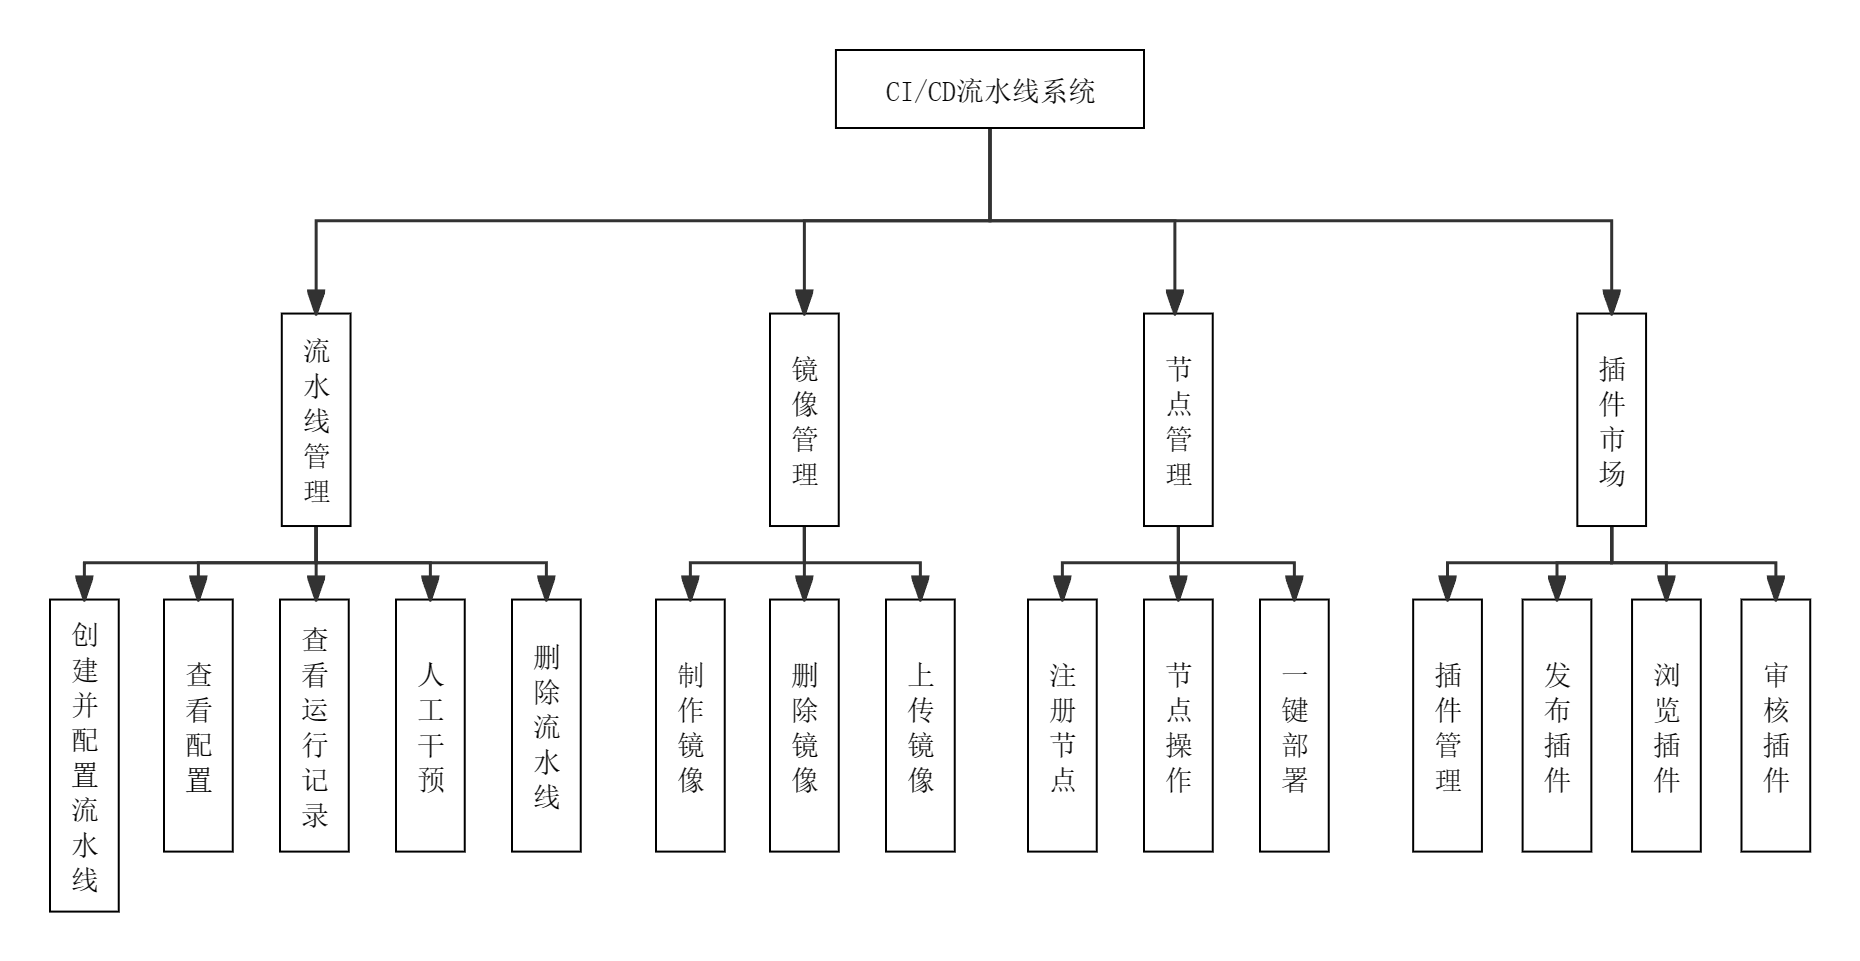
\includegraphics[width=1\textwidth]{功能模块图.png}
  \caption{功能模块图}
  \label{fig:功能模块图}
\end{figure}

\subsection{流水线管理}

\subsubsection{创建并配置流水线}



\subsubsection{触发流水线}

\subsubsection{人工干预流水线}



人工干预流水线时序图如图~\ref{}

\subsection{镜像管理}
\label{subsec:镜像管理}

在基于容器的CI/CD系统中,镜像是构建容器的基础。
在本系统中,如果用户定义一个作业为容器类型时,首先需要选择一个镜像,作业执行时本系统的执行器会根据镜像来创建环境,然后在环境中执行作业中的各个任务。
为保证系统中的容器可以满足不同开发、测试和运维人员人员的需要,系统中应确保有足够多种类的镜像提供给用户选择,所以镜像管理在本系统中至关重要。

在为了实现镜像管理,系统底层区分并提供了两种主要的服务:一是负责存储镜像的仓库服务,二是负责创建镜像的构建服务。
仓库服务负责对镜像文件进行检索和清除,而构建服务则承担着容器运行和镜像创建的职责。
通过这两类服务的协同工作,实现了高效的镜像管理。

以下介绍镜像管理中几个关键功能的设计:

\subsubsection{镜像创建}

该环节生产的镜像将在创建流水线作业的时候所使用,作为流水线作业的初始环境。
一般来讲,镜像的构建需要管理员直接操作物理服务器,通过手动输入Docker命令来完成,这一过程不仅繁琐而且存在安全风险。
在本系统中,镜像的创建过程被移到了在线平台上,用户可以通过Web界面进行镜像创建。系统支持以下两种方式:
\begin{enumerate}
  \item 通过DockerFile文件。这是最常见的构建镜像的方法,用户需要在系统中按照特定语法编写DockerFile,其中可以指定基础镜像、构建命令、端口暴露、文件挂载等。
  这要求用户对DockerFile的编写的语法规则以及shell脚本有所了解。
  \item 通过Commit操作。该方法允许将运行中的容器状态保存为新镜像,此过程中需要基于一个初始镜像启动容器,然后进行环境配置,最终提交更改为新镜像。
\end{enumerate}

这两种方法提供了不同的优势和选择灵活性。其中通过Commit操作的方式需要在用户界面中远程连接到容器,这需要借助基于网页的SSH组件(如Wetty、Guacamole、GateWay等)实现,
本系统中使用Wetty实现用户在Web端与容器内部的交互。

当用户制作镜像时,首先需要填写镜像基础信息,如镜像名、标签等,然后Backend模块会检查数据库中是否有冲突的镜像,如果有则重新返回上一步进行填写。
接下来需要用户选择制作方式,如果用户选择Dockerfile方式,则可以在线编写Dockerfile文件或者直接上传文件,然后镜像制作服务器将调用docker build命令来构建镜像,并返回镜像构建结果;
如果用户选择commit方式,则需要用户选择一个基础镜像,镜像服务器将根据基础镜像调用docker run启动一个容器实例,并暴露出SSH服务的端口,用户在前端通过Wetty进入容器后,进行一系列操作后,
服务器中将调用docker commit将该容器提交为镜像。

镜像制作的活动图如图~\ref{fig:镜像制作活动图}所示。

\begin{figure}[h]
  \centering
  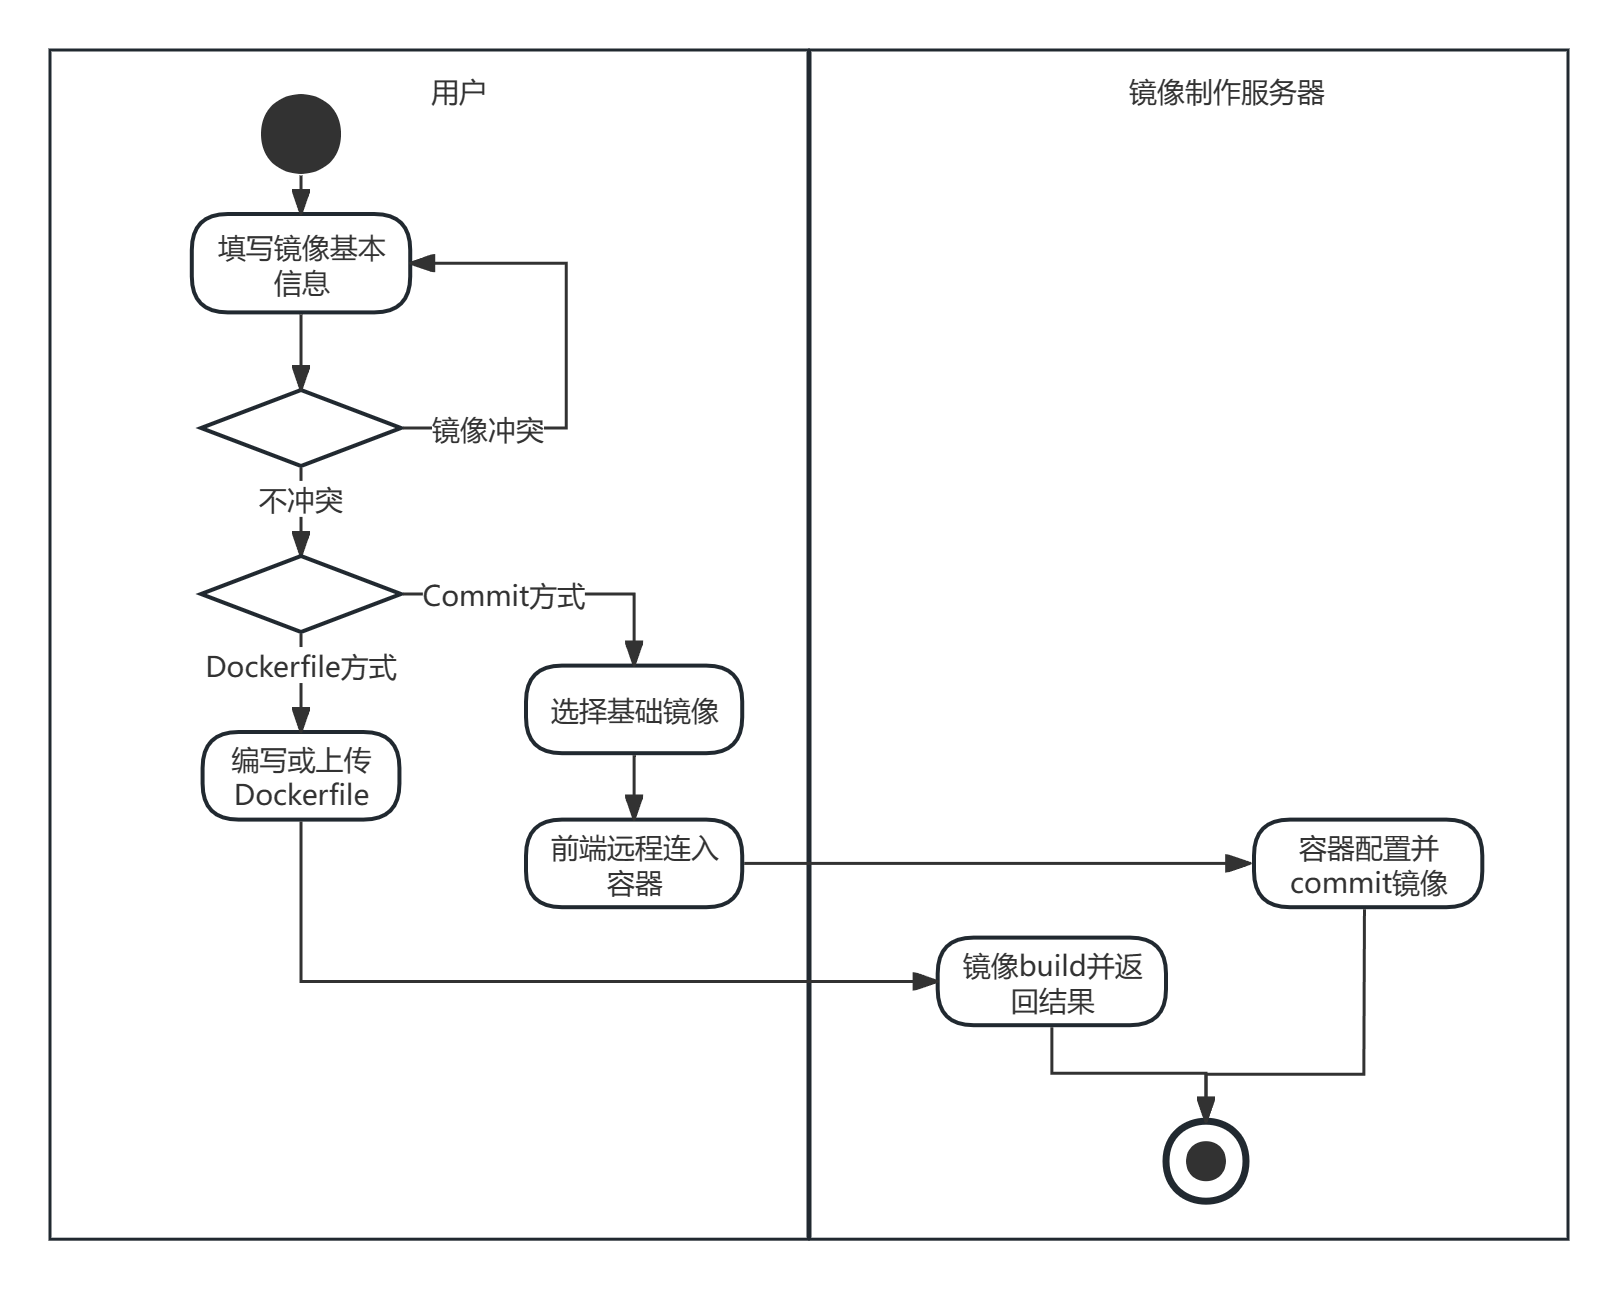
\includegraphics[width=1\textwidth]{镜像制作活动图.png}
  \caption{镜像制作活动图}
  \label{fig:镜像制作活动图}
\end{figure}

\subsubsection{镜像删除}

由于系统中需要支持多样的流水线作业,也就势必需要各种各样的镜像。
随着镜像数量的增加,镜像仓库的存储压力也随之上升,因此需要及时清理不再需要的镜像。

尽管Docker官方提供了删除镜像的API,但该API无法清除所有相关文件。
Docker镜像为了节省存储和带宽,采用了分层构建的机制,镜像的每一层都是基于上一层的更改或添加,每一层都是一个单独的文件。
当一个镜像被推送到系统的镜像仓库,每个镜像会拥有一个Manifest文件,这个文件记录了所有组成本镜像所需要的层。
而当调用Docker API删除一个镜像时,只是删除了镜像所对应的Manifest文件,并不会删除其引用的层,这样就导致有些没有被引用的层残留在仓库中。

如图~ \ref{fig:镜像-Manifest文件-层级关系图}所示,有两个镜像分别对应两个Manifest文件,其中Manifest1引用layer1、layer2、layer3,Manifest1引用layer3和layer4。
当我们调用Docker API删除镜像1后,实际上仓库中被删除的只是Manifest1文件,而此时layer4已经不被任何Manifest文件所引用,但却没有被真正删除。

\begin{figure}[h]
  \centering
  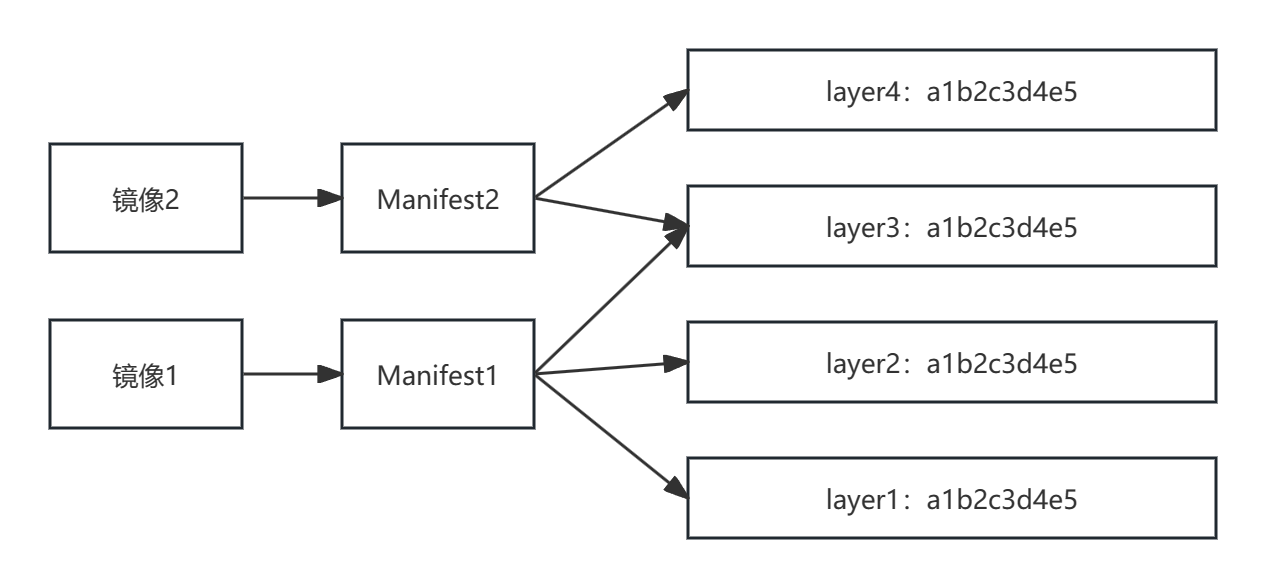
\includegraphics[width=1\textwidth]{镜像层级图.png}
  \caption{镜像-Manifest文件-层级关系图}
  \label{fig:镜像-Manifest文件-层级关系图}
\end{figure}

为解决这一问题,系统中引入了引用计数的功能,这一思想在软件工程中经常被运用,如智能指针、垃圾回收等。
系统将为每一个layer维护其引用计数,当某一层的引用次数降至零时,相应的物理文件也会被删除,从而真正释放存储空间。

镜像删除的活动图如图~\ref{fig:镜像删除活动图}所示。

\begin{figure}[h]
  \centering
  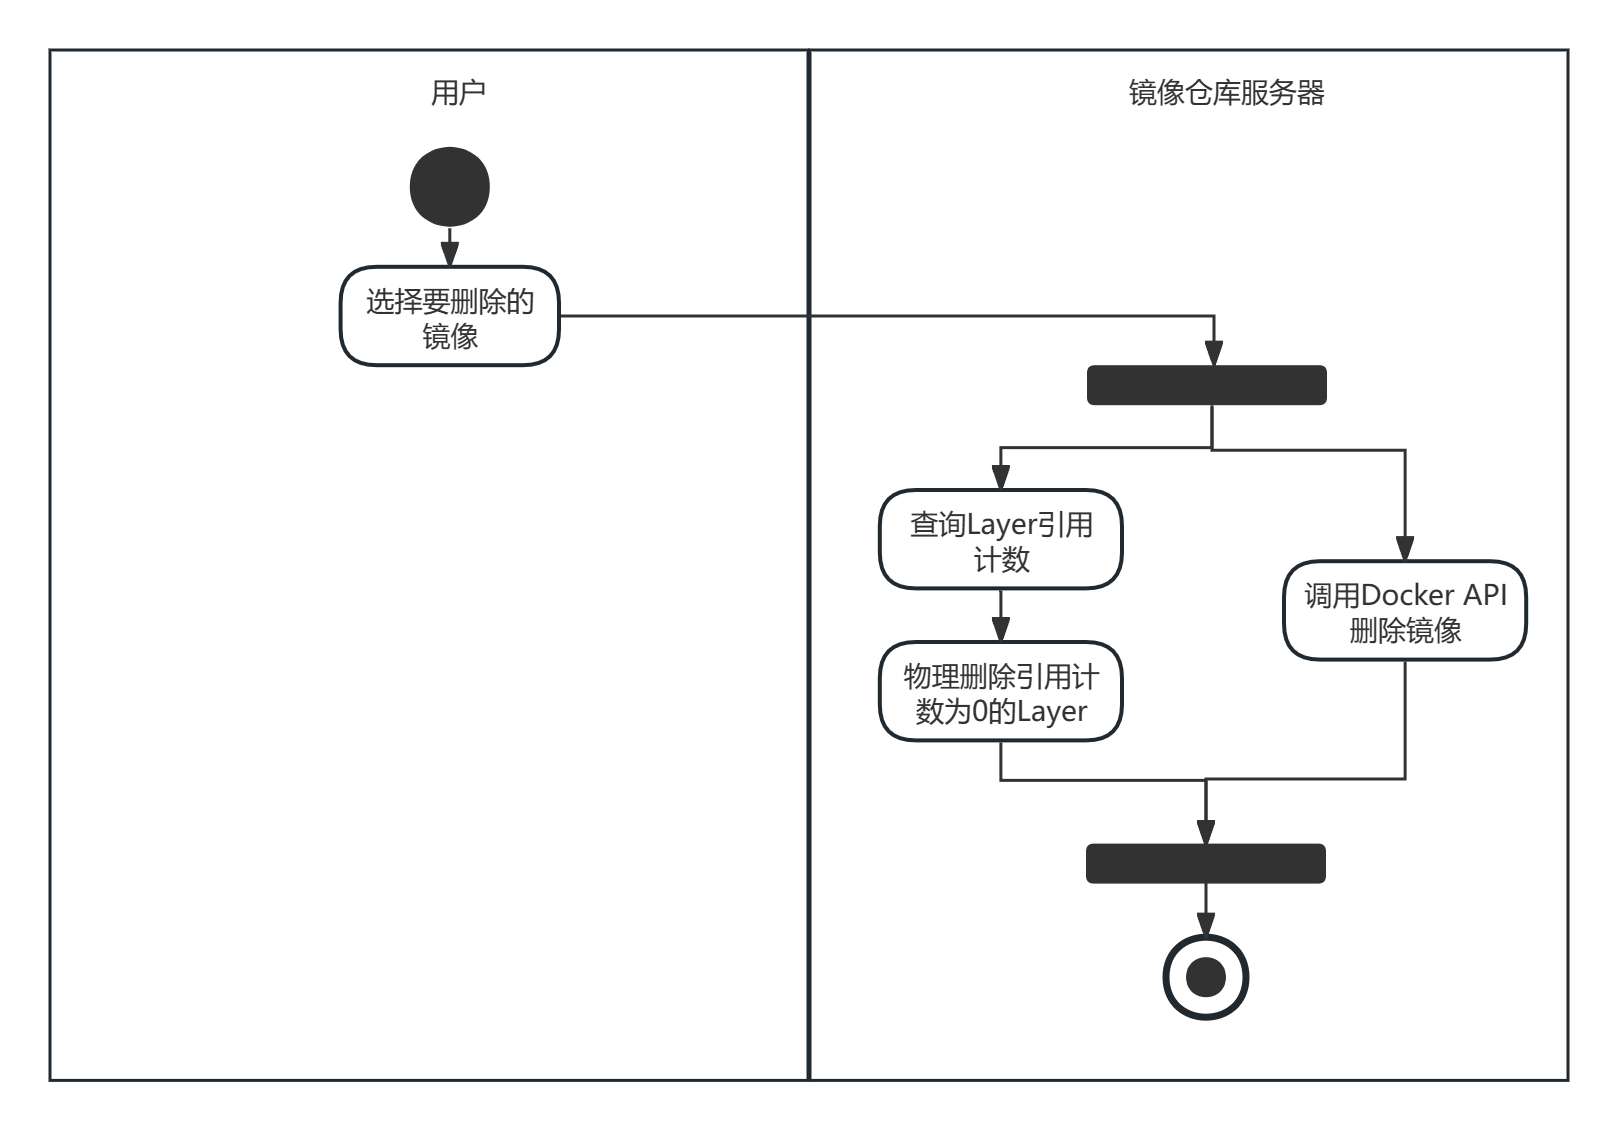
\includegraphics[width=1\textwidth]{镜像删除活动图.png}
  \caption{镜像删除活动图}
  \label{fig:镜像删除活动图}
\end{figure}

\subsubsection{镜像上传}
镜像上传功能使用户能够将创建好的镜像推送至仓库中保存。
考虑到镜像移除功能的改进,上传过程中也需要对层引用记录进行相应的更新,以保持系统数据的一致性和完整性。

在上传镜像时,制作服务器调用Docker API推送镜像至仓库。
镜像制作服务器随后通知仓库服务器更新层引用记录文件。
仓库服务器在接收到更新请求后,检查记录文件状态,并据此更新层引用计数。

\subsection{节点管理}

\subsubsection{节点一键部署}

首先根据用户提供的IP和部署凭证(用户名、密钥或密码)建立SSH连接,然后创建远程目录,以确保存储配置文件和二进制文件的目录存在,
在此之后备份目标服务器上现有的配置文件,创建或打开新的配置文件和系统ID文件,准备写入新的配置,到此为止,节点部署的准备工作完成。
下载并设置执行器的二进制文件,根据提供的配置,生成执行器的配置文件(config.toml)和系统ID文件,编写并配置执行器的systemd服务文件,以便在系统启动时自动启动执行器。
创建或更新/nix目录,并设置为NFS挂载点(如果需要)。通过systemd管理执行器服务:重新加载systemd守护进程,启用并启动执行器服务,最后关闭SSH连接以释放资源。
如果一切顺利,在执行器成功部署后,该服务器便成为了系统中的一个节点,能够与系统主体进行通信并在该节点上执行流水线作业。

节点一键部署活动图如图~ \ref{fig:节点一键部署活动图}所示。

\begin{figure}[h]
  \centering
  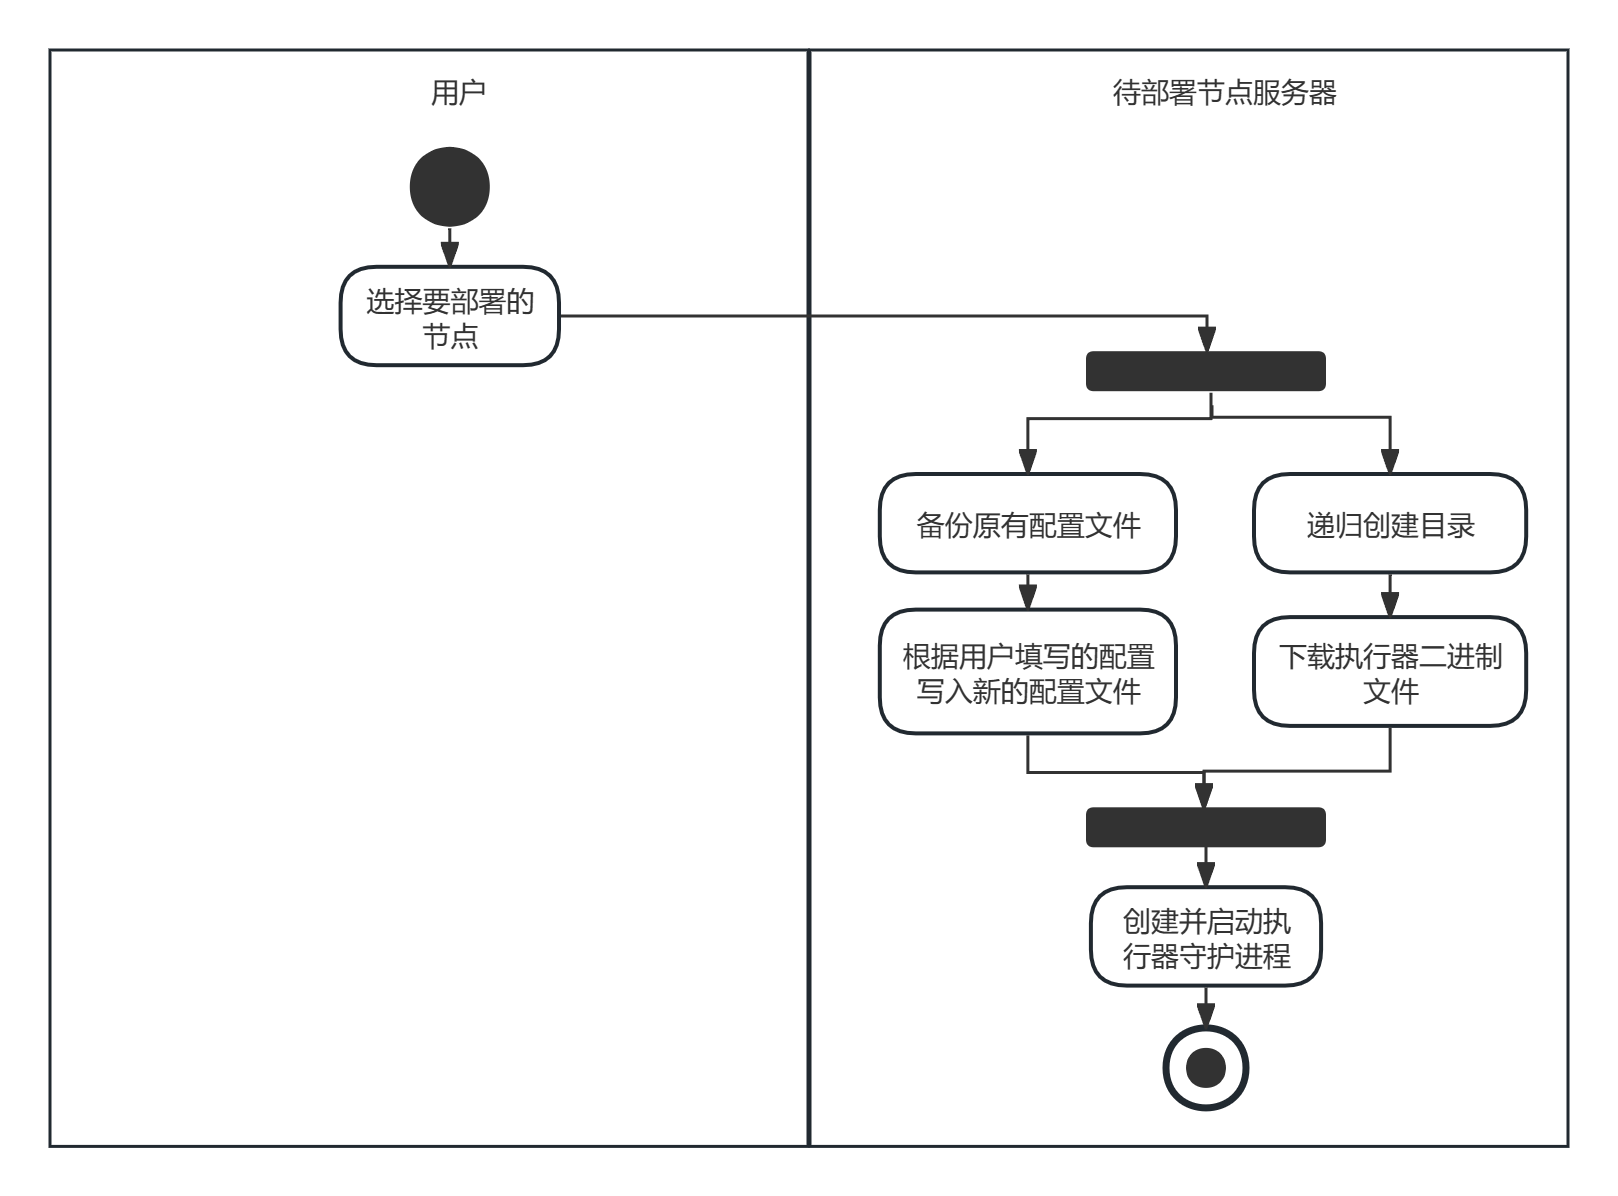
\includegraphics[width=1\textwidth]{节点一键部署活动图.png}
  \caption{节点一键部署活动图}
  \label{fig:节点一键部署活动图}
\end{figure}



\subsection{插件市场}
功能结构图、自动触发hook序列图



\section{数据模型设计}
这一部分将系统中的数据进行抽象,从实体、属性和关系三个维度设计出系统的数据模型,并基于此完成了对数据表的设计。

本系统中的与流水线相关的数据实体可以分为两类,一种是配置(Config)相关实体,一种是运行(RunInfo)相关实体。
同时,由于流水线中存在四个不同层级的子概念,所以本系统中可梳理出2×4=8个与流水线相关的实体:
流水线配置、阶段配置、作业配置、任务配置、流水线运行记录、阶段运行记录、作业运行记录、任务运行记录。

同时,根据前文对需求的整理和分析,系统中还需要对镜像、节点和插件三个概念进行抽象,而节点又是根据Tag标签的方式与作业进行联系的。
所以系统中还应有镜像、节点、节点标签和插件四个实体,加上流水线相关实体,共12个实体。

接下来对实体中的主要属性进行分析,由于流水线相关实体较多且内容具有相似性,此处选取代表性的“作业”相关实体进行分析。

对于作业配置相关实体,应主要包含以下几个方面的属性:
基本信息类包括作业id(主键)、作业所属的阶段id(外键)、名称、创建时间、修改时间、作业位于阶段中的位置;
构建信息类包括,包括 Docker 镜像、输入环境变量;
执行信息类包括:超时时间、触发类型(自动/人工/定时)、是否启用。
可以得到数据库中作业配置表如表~ \ref{tab:作业配置表}

\begin{table}[h]
  \centering
  \caption{作业配置表}
  \label{tab:作业配置表}
  \begin{tabular}{cll}
    \toprule
    字段名                  & 类型            & 描述                                       \\
    \midrule
    id                      & Char           & 主键id                                   \\
    name                    & Char           & 作业名称                                   \\
    trigger\_type           & Char           & 触发方式,自动/手动                        \\
    stage\_config\_id       & ForeignKey     & 关联的阶段配置                             \\
    created\_at             & DateTime       & 创建时间                                    \\
    updated\_at             & DateTime       & 更新时间                                    \\
    image\_id               & ForeignKey     & 关联的Docker镜像                            \\
    variables               & JSON           & 未赋值环境变量                              \\
    tag                     & Char           & 标签                                       \\
    timeout                 & Integer        & 超时时间                                    \\
    position                & Integer        & 位置                                        \\
    run\_condition          & Char           & job的运行条件                               \\
    active                  & Boolean        & 是否启用                                    \\
    version                 & Integer        & 版本号,以追溯修改历史                        \\
    \bottomrule
  \end{tabular}
\end{table}

对于运行记录相关实体,以作业运行记录为例,应包含以下几个方面的属性:
基本信息类包括作业运行记录id(主键)、作业运行记录所属的阶段运行记录id(外键)、作业运行记录所属的作业id(外键);
触发信息类:触发时间、触发人、触发类型;
运行信息类:开始时间、结束时间、作业状态、赋值后的环境变量;
可以得到数据库中作业运行记录表如表~ \ref{tab:作业运行记录表} 所示。

\begin{table}[h]
  \centering
  \caption{作业运行记录表}
  \label{tab:作业运行记录表}
  \begin{tabular}{cll}
    \toprule
    字段名               & 类型          & 描述                                               \\
    \midrule
    job\_config\_id     & ForeignKey   & 关联的作业配置                                     \\
    stage\_run\_info\_id    & ForeignKey   & 关联的阶段运行信息                                 \\
    started\_at         & DateTime     & 作业运行开始时间                                   \\
    end\_at             & DateTime     & 作业运行结束时间                                   \\
    repo\_url           & Char         & 代码仓库URL                                      \\
    repo\_branch        & Char         & 分支名                                           \\
    ref\_sha            & Char         & commit id                                       \\
    variables           & JSON         & 赋值后的环境变量                                  \\
    state               & Char         & 作业的状态,如pending/running/success等            \\
    selected            & Boolean      & 触发时是否勾选,布尔值                             \\
    \bottomrule
  \end{tabular}
\end{table}

其余的流水线配置、阶段配置与任务配置中的属性与作业配置大同小异,此处不再赘述。

然后分析镜像、节点、节点标签和插件四个实体。
对于Docker镜像,有镜像名、镜像ID、镜像描述等基本信息,同时应有镜像标签(Image Label)镜像地址等与镜像存储相关的属性;
节点的本质是一个服务器,应包含服务器信息,如服务器IP、端口号、主机名、登录凭证等,同时也应包含节点名称、节点描述等基本信息。
节点标签是不同作业分配到不同节点上的依据,同时又是节点与作业多对多关系的中间表,包含名称、节点ID、作业ID等属性;
插件作为任务的模板,包含了大部分任务实体中的属性,如脚本内容、环境变量等,同时包含一些插件特有的属性,如版本号、配置表单、插件logo等。

最后分析系统内实体之间的关系。一个配置的一次执行即产生了一个运行实例,这与编程语言中“类”和“类对象”的关系类似,
即“运行”是“配置”的实例化,“配置”是“运行”的模板,因此配置与运行是一对多的关系。
同时根据流水线的各个子概念的定义,我们知道有:流水线与阶段是一对多的关系,阶段与作业是一对多的关系,作业与任务是一对多的关系。
由于作业中包含镜像,所以镜像与作业是一对多的关系。
每个作业需要指定一个节点或多个节点,每个节点又可以被多个作业所指定,所以作业与节点是多对多的关系,作业标签自然就是作业与节点的中间表。
插件由于是任务的模板,所以与任务是一对多的关系,一个插件可以应用于多个任务,一个任务只能指定一个插件。

结合以上分析,可得出系统的实体-关系图(E-R图)如图~\ref{fig:系统E-R图}:

\begin{figure}[h]
  \centering
  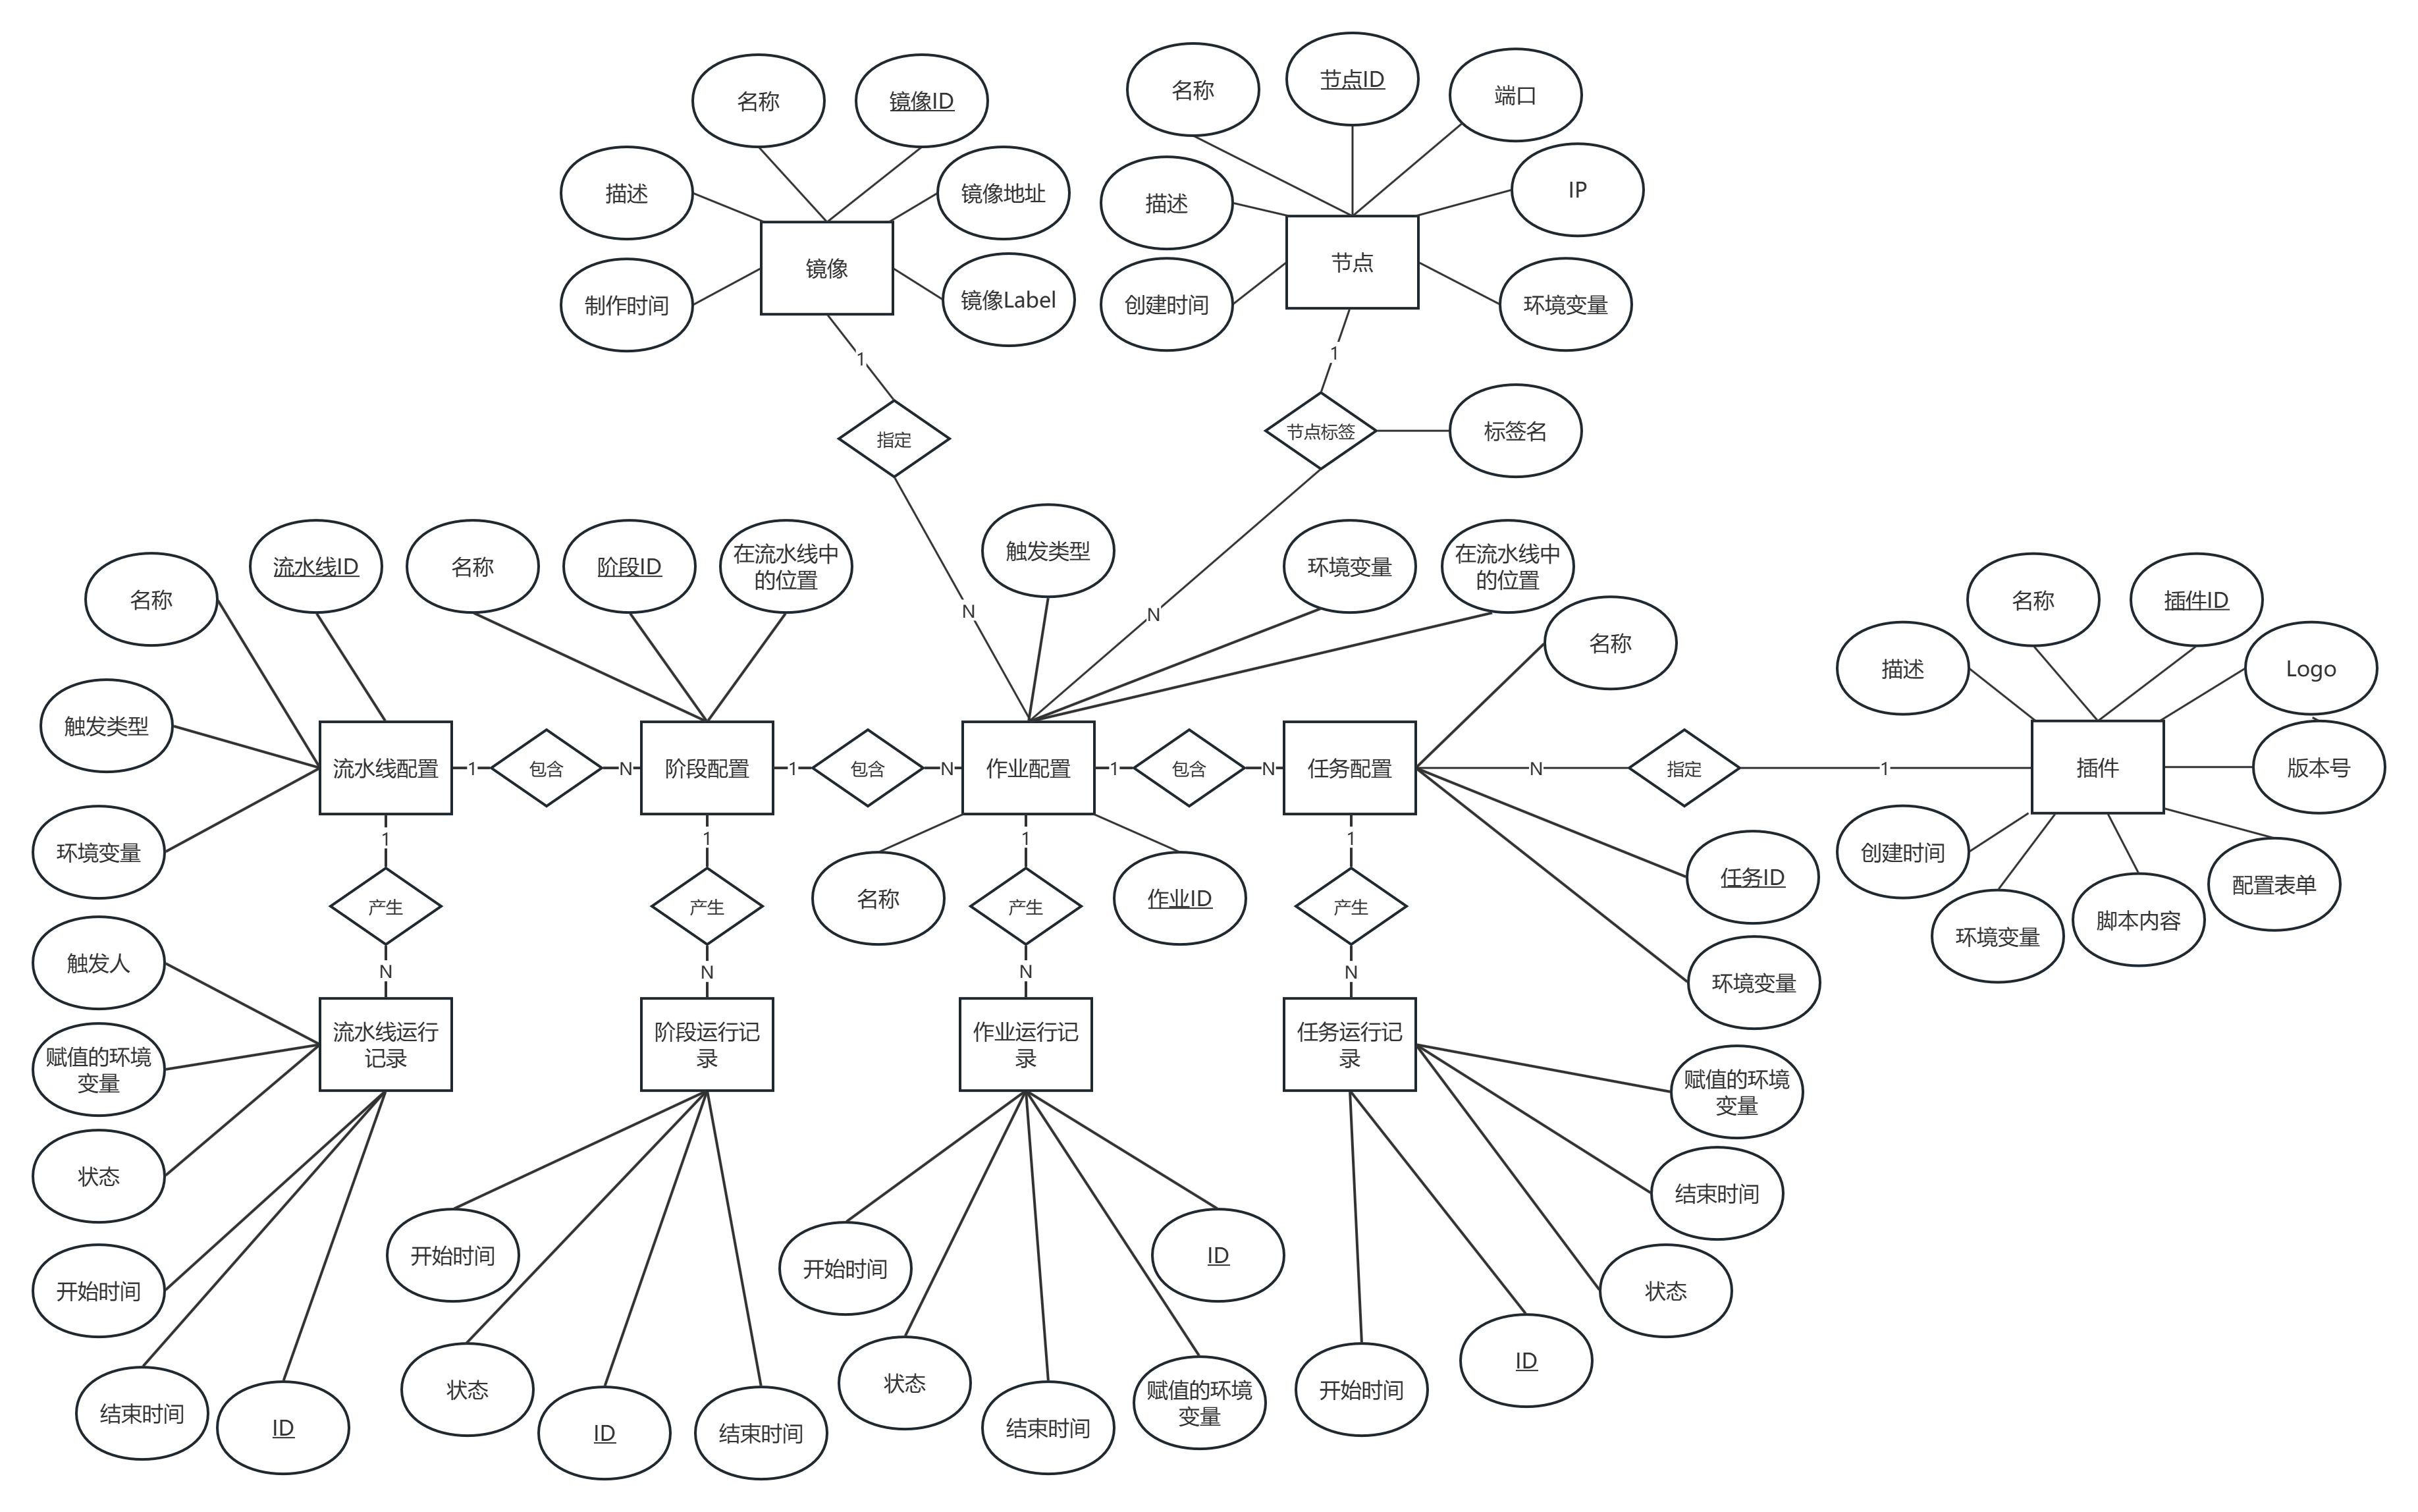
\includegraphics[width=1\textwidth]{系统ER图.png}
  \caption{系统E-R图}
  \label{fig:系统E-R图}
\end{figure}


